\section{Thermal Hydraulics}
\label{sec:thermalHydraulics}

\begin{frame}{Material Properties}
  \begin{itemize}
    \item Functional sodium properties from \cite{sodiumProp}.
    \item Clad and sodium thermal conductivity assumed constant \cite{ht9Prop}.
    \item Fuel thermal conductivity assumed a function of temperature
      \cite{fuelProp}.
  \end{itemize}
  \begin{table}
    \caption{Constant Thermal Conductivity for Sodium and HT9.}
    \label{tab:constant_k}
    \begin{center}
      \begin{tabular}{cl}
        \toprule
        Material & $k \units{$\frac{\text{W}}{\text{m K}}$}$ \\
        \midrule
        Sodium &  64.33 \\
        HT9    &  25.81 \\
        \bottomrule
      \end{tabular}
    \end{center}
  \end{table}
\end{frame}

\begin{frame}{Fuel Thermal Conductivity}
  \begin{align}
    \label{eq:kfuel_first}
    k_U      &= 21.73 + 1.591 \times 10^{-2} T + 5.907 \times 10^{-6} T^2 \\
    k_{Zr}   &= 8.853 + 7.082 \times 10^{-3} T + 2.533 \times 10^{-6} T^2 +
      2.992 \times 10^{3} T^{-1} \\
    k_{c,Zr} &= -102.0 + 200.1 x_{Zr} - 109.2 x_{Zr}^2 + 
      9.435 \times 10^{-3} T + 3.459 \times 10^{-5} T^2 - 0.02093 x_{Zr} \, T \\
    \label{eq:kfuel_last}
    k_{U-Zr} &= \left( 1 - \sqrt{1-x_{Zr}}\right) k_{Zr} + 
      \sqrt{1 - x_{Zr}} \left( \left( 1 - x_{Zr}\right) k_U + x_{Zr} \, k_{c,Zr}
      \right) 
  \end{align}
  \begin{figure}
    \centering
    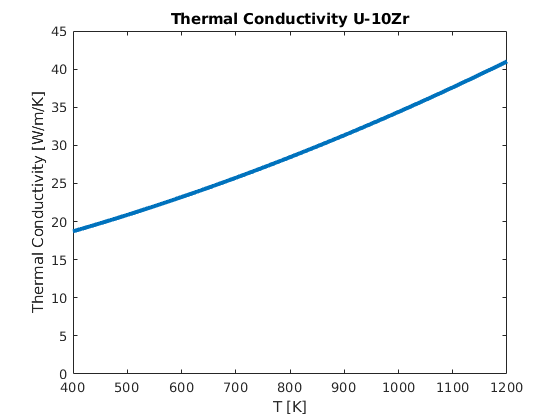
\includegraphics[width=0.5\textwidth]{kfuel_plot}
    %\caption{Variable Thermal Conductivity in Fuel.}
    \label{fig:kfuel_plot}
  \end{figure}
\end{frame}

\begin{frame}{Axial Convection Geometric Model}
  \begin{columns}
    \begin{column}{0.5\textwidth}
      \begin{figure}
        \centering
        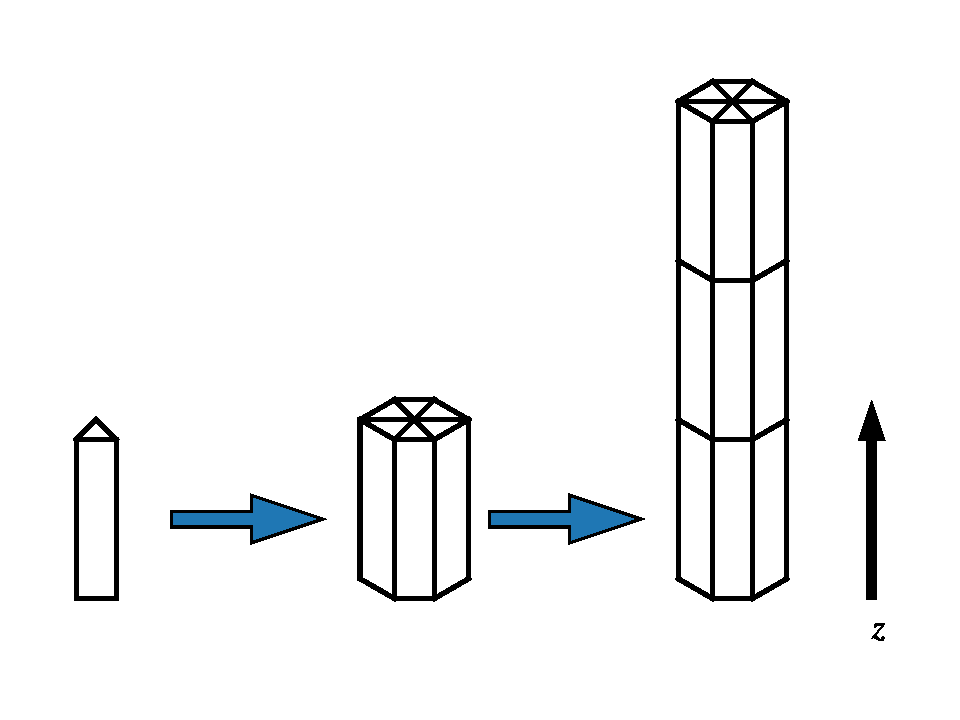
\includegraphics[width=\textwidth]{chunk_description}
        \caption{Progression of Element (left), to Chunk (center), to Channel
          (right).}
        \label{fig:chunk_description}
      \end{figure}
    \end{column}
    \begin{column}{0.5\textwidth}
      \begin{figure}
        \centering
        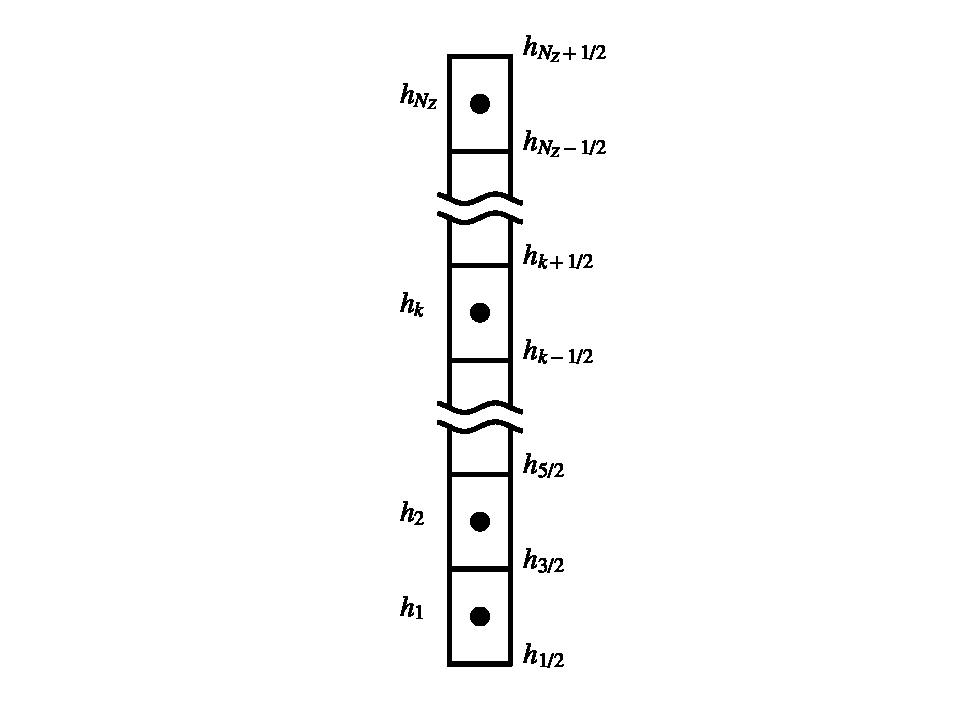
\includegraphics[width=0.35\textwidth]{axial_model}
        %\caption{One-Dimensional Axial Heat Convection Model Description.}
        \label{fig:axial_model}
      \end{figure}
    \end{column}
  \end{columns}
\end{frame}

\begin{frame}{Channel Enthalpy}
  Steady-state coolant enthalpy within the channel is given by an energy
  balance.
  \begin{equation}
    \label{eq:continuous_heat_balance}
    h_i(z) = h_{in} + \frac{1}{\mdot_i} \int_0^z q'_i(z') \; dz'
  \end{equation}
  $h_{in}$ is given by a state relationship from a user-input $T_{inlet}$.
  \begin{equation}
    h_{in} = h(T_{inlet})
  \end{equation}
  Discretize the integral to calculate the enthalpy at the upper node of the
  chunk.
  \begin{equation}
    h_{i,k+1/2} = h_{in} + \frac{1}{\mdot_i} \sum_{k=1}^{N_z} q_{i,k}
  \end{equation}
  Use a first-order approximation to estimate the chunk-average enthalpy.
  \begin{equation}
    h_{i,k} = \half (h_{i,k-1/2}+h_{i,k+1/2})
  \end{equation}
  $T_{\infty,i,k}$ is then given by a state relationship \cite{sodiumProp}.
  \begin{equation}
    T_{\infty,i,k} = T(h_{i,k})
  \end{equation}
\end{frame}

\begin{frame}{Radial Conduction Geometric Model}
  \begin{figure}
    \centering
    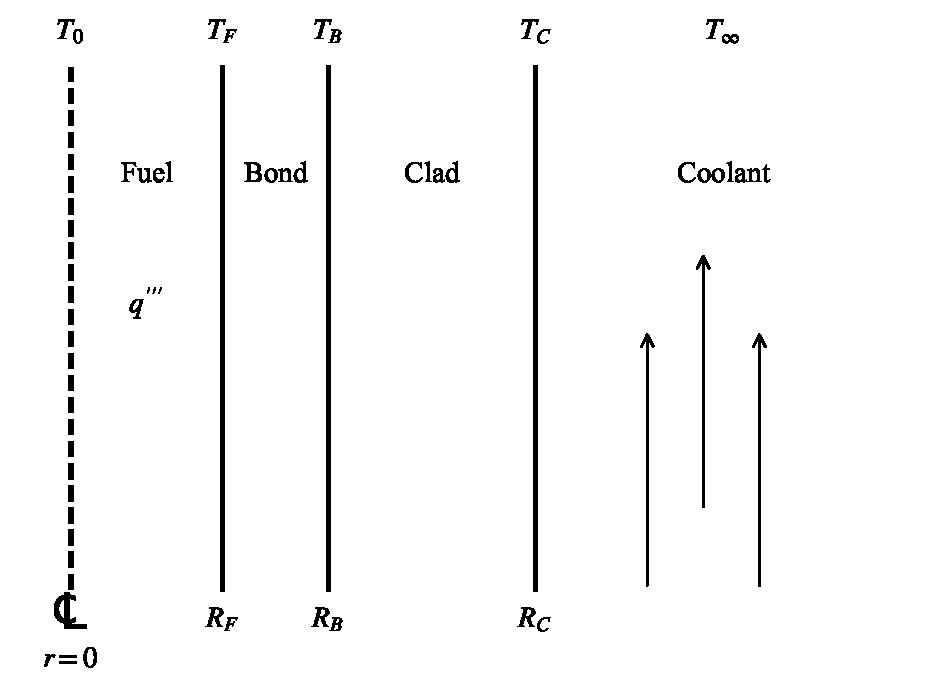
\includegraphics[width=0.7\textwidth]{radial_model}
    \caption{Geometry Description of Radial Heat Conduction Model (not to
      scale).}
    \label{fig:radial_model}
  \end{figure}
\end{frame}

\begin{frame}{Radial Assumptions}
  \begin{itemize}
    \item Axial conduction is negligible within solid materials.
    \item Constant volumetric heat conduction rate within the fuel.
  \end{itemize}
\end{frame}

\begin{frame}{Clad Surface Temperature -- Subbotin-Ushakov}
  Using Newton's Law of Cooling.
  \begin{align}
    q''_{clad} &= H_c (T_C - T_{\infty}) \\
    q''_{ckad} &+ q'''_{i,k} \frac{R_F^2}{2 R_C}
  \end{align}
  $H_c$ is given by the Subbotin-Ushakov correlation \cite{subbotinUshakov}
  which relates the Nusselt and P\'eclet numbers.
  \begin{align}
    Pe &= Re \, Pr \\
    \label{eq:subbotinUshakov}
    Nu &= 7.55 \frac{S}{D} - 20 \left(\frac{S}{D}\right)^{-13} + 
      \frac{3.67}{90\left(\frac{S}{D}\right)^{2}}
      Pe^{\left(0.56 + 0.19 \frac{S}{D}\right)}
  \end{align}
  Then the clad surface temperature, $T_C$ follows.
  \begin{align}
    H_c &= \frac{N\!u \, k}{D_e} \\
    T_C &= \frac{q''_{clad}}{H_c} + T_{\infty}
  \end{align}
\end{frame}
